\subsection{Thiết kế Sitemap}

\begin{figure}[H]
	\centering
	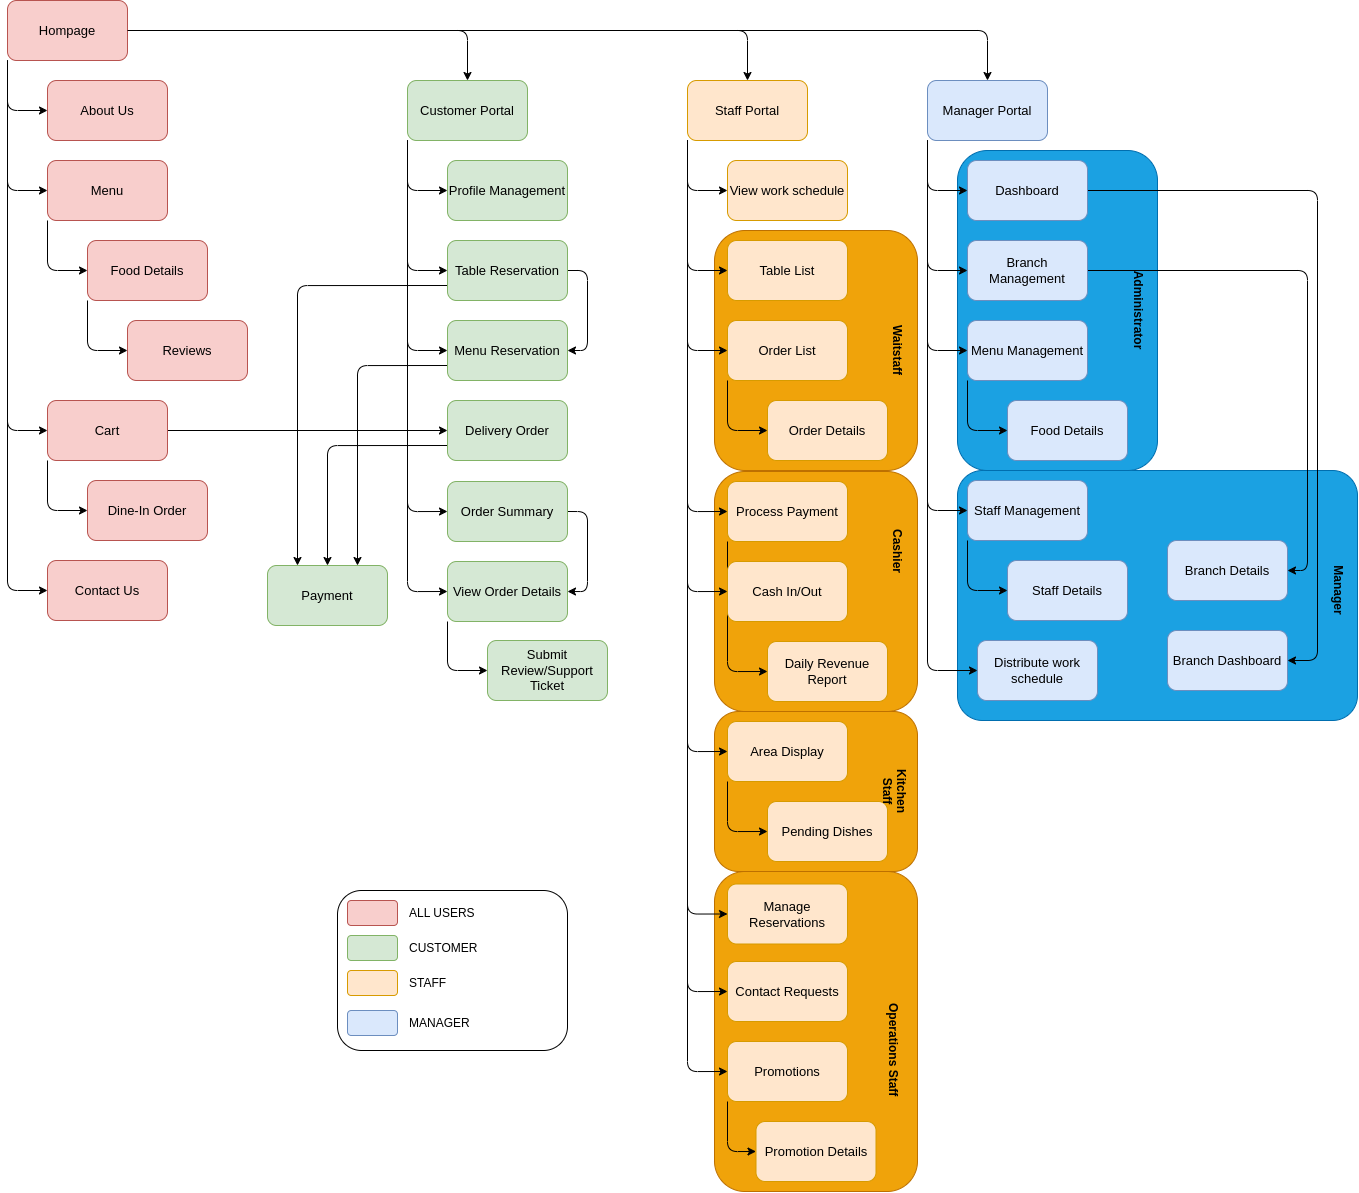
\includegraphics[width=\linewidth]{Images/sitemap.png}
	\vspace{0.5cm}
	\caption{Sitemap của hệ thống}
	\label{fig:my_label}
\end{figure}

Sitemap này mô tả cấu trúc và các tính năng chính của Hệ thống quản lý đặt món cho nhà hàng, nêu chi tiết các chức năng và mô-đun cốt lõi của nó.

\begin{enumerate}
	\item \textbf{Tất cả người dùng}
	      \begin{itemize}
		      \item \textit{Homepage}: Trang chính của ứng dụng, hiển thị thông tin giới thiệu về nhà hàng, các danh mục chính (Menu, Đặt hàng, Liên hệ), và nút đăng nhập/đăng ký để chuyển đến các cổng phù hợp với vai trò người dùng.
		      \item \textit{About Us (Giới thiệu)}: Cung cấp thông tin về nhà hàng, bao gồm lịch sử, giá trị cốt lõi, đội ngũ, và các chi nhánh.
		      \item \textit{Menu}: Hiển thị danh sách các món ăn và khuyến mãi hiện có, phân loại theo loại (đồ ăn, đồ uống, món tráng miệng), cho phép người dùng xem chi tiết món ăn và thêm vào giỏ hàng.
		      \item \textit{Food Details (Chi tiết món ăn)}: Food Details (Chi tiết món ăn): Hiển thị thông tin chi tiết về một món ăn cụ thể (tên, giá, mô tả, hình ảnh, thành phần, đánh giá), cho phép thêm vào giỏ hàng hoặc quay lại danh sách menu.
		      \item \textit{Cart (Giỏ hàng)}: Hiển thị danh sách món ăn đã chọn, cho phép chỉnh sửa số lượng và ghi chú, xóa món, và chọn phương thức đặt hàng (Dine-In Order hoặc Delivery Order).
		      \item \textit{Dine-In Order (Đặt món tại quán)}: Cho phép người dùng xác nhận đơn hàng để ăn tại quán, cho phép chuyển sang trang thanh toán khi hoàn thành bữa ăn.
		      \item \textit{Payment (Thanh toán)}: Xử lý thanh toán cho đơn hàng tại quán, hỗ trợ các phương thức thanh toán (tiền mặt, thẻ, QR code), và hiển thị xác nhận sau khi thanh toán thành công.
		      \item \textit{Contact Us (Liên hệ)}: Cung cấp thông tin liên hệ (số điện thoại, email, địa chỉ), và biểu mẫu để khách hàng gửi câu hỏi hoặc phản hồi.
	      \end{itemize}
	\item \textbf{Khách hàng đã có tài khoản}
	      \begin{itemize}
		      \item \textit{Profile Management (Quản lý thông tin cá nhân)}: Cho phép khách hàng xem và chỉnh sửa thông tin cá nhân (tên, số điện thoại, email, địa chỉ), quản lý tài khoản và mật khẩu.
		      \item \textit{Table Reservation (Đặt bàn)}: Cho phép khách hàng chọn thời gian, số lượng người, xem sơ đồ và đặt bàn tại nhà hàng, với xác nhận qua email hoặc tin nhắn. Nếu đang có yêu cầu đặt bàn thì cũng sẽ hiển thị và hủy ở đây.
		      \item \textit{Delivery Order (Đặt món giao về)}: Cho phép người dùng chọn giao hàng, nhập thông tin giao hàng (địa chỉ, số điện thoại), và chuyển sang trang thanh toán.
		      \item \textit{Order Summary (Tóm tắt đơn hàng)}: Hiển thị tất cả đơn hàng (món ăn, số lượng, tổng tiền, thông tin giao hàng), cho phép chuyển qua trang xem chi tiết.
		      \item \textit{View Order Details (Xem chi tiết đơn hàng)}: Hiển thị trạng thái và thông tin chi tiết của một đơn hàng đã đặt (thời gian, địa chỉ, tình trạng giao hàng), cho phép khách hàng theo dõi. Nếu đơn hàng đã thành công, có thể chuyển đến trang gửi đánh giá.
		      \item \textit{Submit Review (Gửi đánh giá)}: Cho phép người dùng viết đánh giá hoặc xếp hạng cho món ăn hoặc dịch vụ sau khi hoàn tất đơn hàng, gửi lên hệ thống.
	      \end{itemize}
	\item \textbf{Nhân viên}

	      \textbf{\textit{Tất cả nhân viên}}
	      \begin{itemize}
		      \item \textit{View word schedule (Xem lịch làm)}: Hiển thị lịch làm việc được xếp.
	      \end{itemize}
	      \textbf{\textit{Nhân viên Phục vụ}}
	      \begin{itemize}
		      \item \textit{Table List (Danh sách bàn)}: Hiển thị trạng thái các bàn (trống, đang sử dụng, đặt trước), cho phép nhân viên phục vụ cập nhật hoặc quản lý.
		      \item \textit{Order List (Danh sách đơn hàng)}: Hiển thị danh sách các đơn hàng đang chờ xử lý, cho phép nhân viên chọn đơn để xem chi tiết hoặc chuyển sang bếp.
		      \item \textit{Order Details (Chi tiết đơn hàng)}: Hiển thị thông tin chi tiết của một đơn hàng (món ăn, số lượng, ghi chú), cho phép nhân viên xác nhận hoặc cập nhật trạng thái.
	      \end{itemize}

	      \textit{\textbf{Nhân viên Thu ngân}}
	      \begin{itemize}
		      \item \textit{Process Payment (Xử lý thanh toán)}: Cho phép nhân viên thu ngân nhập thông tin thanh toán, xử lý các phương thức (tiền mặt, thẻ), và xuất hóa đơn.
		      \item \textit{Cash In/Out}: Thêm thông tin vào dòng tiền bên ngoài.
		      \item \textit{Daily Revenue Report (Báo cáo doanh thu hàng ngày)}: Hiển thị tổng doanh thu, số lượng đơn hàng, và các thống kê khác trong ngày, hỗ trợ nhân viên thu ngân theo dõi.
	      \end{itemize}

	      \textit{\textbf{Nhân viên Bếp}}
	      \begin{itemize}
		      \item \textit{Area Display (Các khu vực bếp): Hiển thị danh sách các khu vực bếp tương ứng với các món ăn được chỉ định sẵn.}
		      \item \textit{Pending Dishes (Món ăn đang chờ)}: Hiển thị danh sách món ăn cần chuẩn bị, cho phép nhân viên bếp theo dõi và cập nhật trạng thái hoàn thành.
	      \end{itemize}

	      \textit{\textbf{Nhân viên Vận hành}}
	      \begin{itemize}
		      \item \textit{Manage Reservations (Quản lý đặt bàn)}: Cho phép nhân viên xem, chỉnh sửa, hoặc hủy đặt bàn (bao gồm hủy khi khách đến trễ quá), cập nhật trạng thái bàn.
		      \item \textit{Contact Requests (Yêu cầu liên hệ)}: Hiển thị danh sách yêu cầu hỗ trợ từ khách hàng, cho phép nhân viên hỗ trợ trả lời hoặc chuyển tiếp.
		      \item \textit{Promotions (Khuyến mãi)}: Hiển thị danh sách các chương trình khuyến mãi hiện tại, cho phép quản lý tạo mới hoặc chỉnh sửa.
		      \item \textit{Promotion Details (Chi tiết khuyến mãi)}: Hiển thị thông tin chi tiết của từng chương trình khuyến mãi (thời gian, điều kiện, ưu đãi), cho phép chỉnh sửa hoặc xóa. Thống kê số liệu về chương trình khuyến mãi
	      \end{itemize}
	\item \textbf{Quản lý}
	      \begin{itemize}
		      \item \textit{Staff Management (Quản lý nhân viên)}: Cho phép quản lý thêm, chỉnh sửa, hoặc xóa thông tin nhân viên (tên, vai trò, lịch làm việc).
		      \item \textit{Staff Details (Chi tiết nhân viên)}: Hiển thị thông tin chi tiết của từng nhân viên (hồ sơ, lịch sử làm việc, hiệu suất), cho phép chỉnh sửa.
		      \item \textit{Branch Details (Chi tiết chi nhánh)}: Hiển thị thông tin chi tiết của chi nhánh, cho phép chỉnh sửa sơ đồ nhà hàng.
		      \item \textit{Branch Dashboard (Bảng điều khiển chi nhánh)}: Hiển thị thông tin cụ thể của từng chi nhánh (doanh thu, đơn hàng, nhân viên), hỗ trợ quản lý theo dõi.
		      \item \textit{Distribute work schedule (Xếp lịch làm)}: Cho phép lập lịch trực qua, thêm ghi chú công việc cho nhân viên.
	      \end{itemize}

	      \textit{\textbf{Dành cho quản trị viên}}
	      \begin{itemize}
		      \item \textit{Dashboard (Bảng điều khiển)}: Hiển thị tổng quan về hoạt động nhà hàng (doanh thu, số đơn hàng, trạng thái nhân viên), với các biểu đồ và số liệu chính.
		      \item \textit{Branch Management (Quản lý chi nhánh)}: Cho phép quản lý thêm, chỉnh sửa, hoặc xóa thông tin chi nhánh (địa chỉ, số điện thoại, giờ hoạt động).
		      \item \textit{Menu Management (Quản lý menu)}: Cho phép quản lý thêm, chỉnh sửa, hoặc xóa món ăn trong menu (tên, giá, hình ảnh, mô tả). Thống kế các thông tin số liệu về món ăn.
		      \item \textit{Food Details (Chi tiết món ăn)}: Hiển thị và chỉnh sửa thông tin chi tiết của từng món ăn trong menu (dành cho quản lý).
	      \end{itemize}

\end{enumerate}

\subsection{Thiết kế Database}
\subsubsection{EERD Database}

Hệ thống cơ sở dữ liệu quản lý một chuỗi nhà hàng, tập trung vào việc quản lý người dùng, nhân viên, khách hàng, đặt bàn, gọi món, hóa đơn thanh toán, chương trình khuyến mãi, phản hồi và hỗ trợ khách hàng. Người dùng (USER) lưu trữ các thông tin như tên đăng nhập, mật khẩu đã mã hóa, họ tên đầy đủ và địa chỉ email. Một người dùng có thể là một nhân viên (STAFF), đảm nhiệm các vai trò như thu ngân (CASHIER), đầu bếp (CHEF), nhân viên phục vụ (WAITER), nhân viên vệ sinh (CLEANING STAFF), nhân viên vận hành (OPERATION STAFF). Người dùng cũng có thể là quản lý (MANAGER) hoặc khách hàng (CUSTOMER). Mỗi nhân viên bắt buộc phải làm việc tại một chi nhánh (BRANCH) cụ thể. Mỗi chi nhánh lưu trữ các thông tin về tên, địa chỉ và số điện thoại liên hệ, đồng thời phải có một bản cấu hình (CONFIGURATION) riêng biệt để thiết lập các chính sách như tiền đặt cọc bàn, tỷ lệ đặt cọc khi đặt món trước, thời gian tự động gọi xác nhận đơn hàng hoặc các thông số kỹ thuật khác. Mỗi chi nhánh có đúng một người quản lý (MANAGER) chịu trách nhiệm vận hành toàn bộ hoạt động tại chi nhánh đó.

Nhân viên làm việc theo ca (SHIFT), mỗi ca ghi nhận giờ bắt đầu, giờ kết thúc, ghi chú đặc biệt nếu có và trạng thái như nháp, xung đột, hoàn thành hoặc đã lên lịch. Nhân viên nhà bếp sẽ được phân công làm việc tại các khu vực bếp (KITCHEN STATION) thuộc từng chi nhánh riêng biệt, mỗi khu vực bếp có tên và mô tả cụ thể. Một chi nhánh phải có ít nhất một khu vực bếp được cấu hình trước khi có thể bắt đầu vận hành.

Nhà hàng bố trí nhiều bàn ăn (TABLE) với các thông tin về số lượng chỗ ngồi và vị trí cụ thể trên bản đồ nhà hàng. Bàn có các trạng thái vận hành như trống, đang sử dụng hoặc chờ làm sạch. Khách hàng có thể thực hiện việc đặt bàn trước (BOOKING TABLE), ghi lại số lượng khách, thời gian ăn, các ghi chú thêm và trạng thái đặt bàn như đã xác nhận, đã hủy hoặc thành công. Khách hàng cũng có thể đặt món trước (BOOKING DISH), ghi nhận các món ăn mong muốn, số lượng từng món, thời gian ăn dự kiến tới ăn và ghi chú riêng cho từng món nếu cần.

Món ăn (DISH) lưu trữ thông tin về tên món, mô tả, kích cỡ phần ăn, giá tiền, thời gian chế biến ước tính và trạng thái hoạt động. Mỗi món ăn được tạo thành từ nhiều nguyên liệu. Ngoài ra, nhà hàng còn xây dựng các combo (COMBO) kết hợp nhiều món ăn với giá ưu đãi để bán cho khách.

Khi khách hàng gọi món hoặc đặt món, hệ thống tạo ra đơn hàng (ORDER) với thông tin loại đơn (ăn tại chỗ, mang đi, giao hàng), trạng thái đơn hàng (thành công, đang thực hiện, đã hủy...), tiền cọc nếu có và tổng giá trị đơn hàng, được tính bằng cách lấy giá từng món ăn hoặc combo (áp dụng giá khuyến mãi nếu có) nhân với số lượng rồi cộng lại. Đối với đơn giao hàng sẽ có thêm thông tin vận chuyển. Mỗi đơn hàng có thể gắn với một hoặc nhiều hóa đơn (INVOICE) trong trường hợp chia nhỏ hóa đơn, ghi lại tổng số tiền thanh toán (sau khi áp dụng voucher nếu có, trừ đi tiền cọc), thuế VAT, thời gian lập hóa đơn và loại hóa đơn (hóa đơn gộp hoặc hóa đơn lẻ). Khách hàng thanh toán qua các phương thức thanh toán (PAYMENT) khác nhau như tiền mặt, ví điện tử hoặc ebanking. Các khoản đặt cọc cho đặt bàn hoặc đặt món cũng được ghi nhận dưới dạng PAYMENT riêng biệt, với số tiền tính theo phần trăm cấu hình tại CONFIGURATION.

Hệ thống quản lý các mã giảm giá (VOUCHER), mỗi voucher có điều kiện áp dụng cụ thể, giới hạn số lần sử dụng, thời gian hiệu lực, lưu lại số phần trăm giảm giá hoặc số tiền giảm giá. Khách hàng có thể lưu trữ các voucher được phát hành để sử dụng về sau nếu voucher còn hiệu lực. Ngoài voucher, nhà hàng còn có các chương trình khuyến mãi (PROMOTION) diễn ra trong các khoảng thời gian xác định, giảm giá trực tiếp trên món ăn.

Khách hàng có thể gửi yêu cầu hỗ trợ (SUPPORT TICKET) với tiêu đề, nội dung cụ thể và trạng thái xử lý như đã xử lý, đang xử lý hoặc đang chờ bổ sung thông tin. Mỗi yêu cầu sẽ được phân công cho nhân viên vận hành để tiếp nhận và xử lý. Khách hàng cũng có thể gửi phản hồi (FEEDBACK) với nội dung giới hạn trong 500 ký tự về dịch vụ hoặc món ăn, gắn liền với từng đơn hàng, và đánh giá chất lượng từ 1 đến 5 sao. Trong trường hợp có sự cố, khách hàng có thể yêu cầu hoàn tiền (REFUND), yêu cầu này gắn liền với hóa đơn (INVOICE) liên quan để nhân viên có thể theo dõi và xử lý.

\begin{landscape}
	\begin{figure}[H]
		\centering
		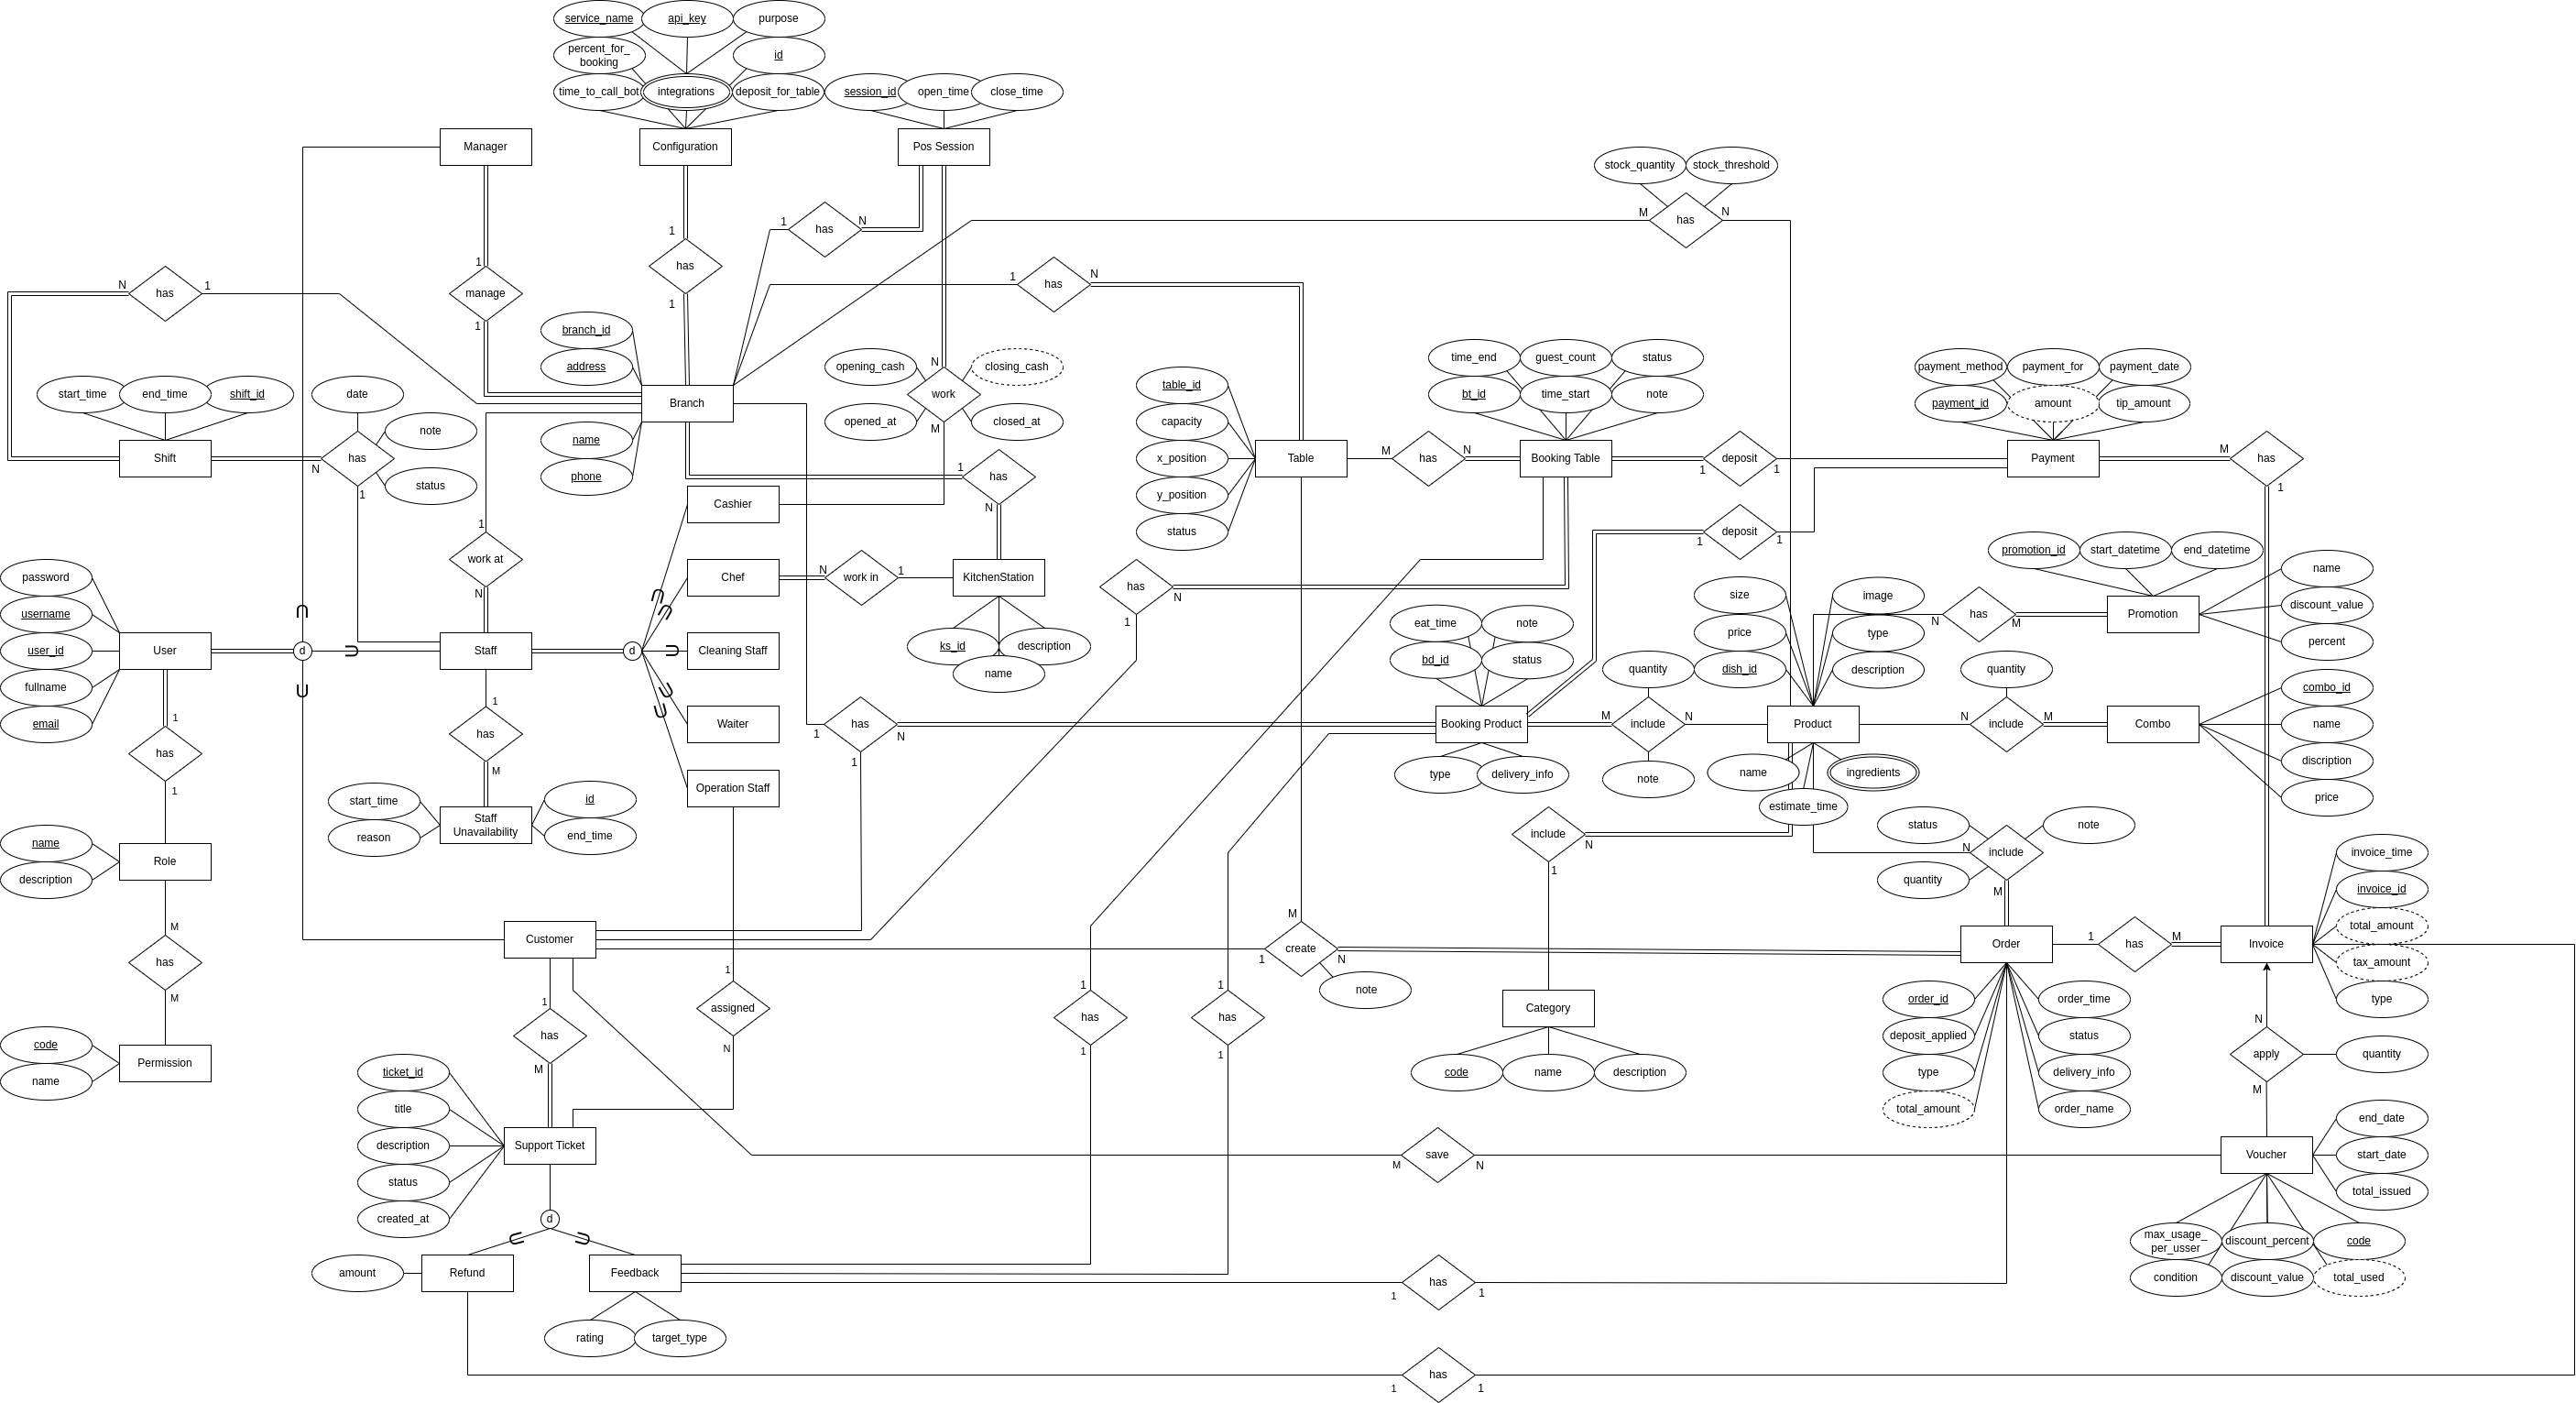
\includegraphics[height=0.85\textheight]{Images/db.png}
		\vspace{0.5cm}
		\caption{EERD của cơ sở dữ liệu}
		\label{fig:my_label}
	\end{figure}
\end{landscape}

% \subsubsection{Các ràng buộc}
% \paragraph{Ràng buộc miền trị (Domain Constraints – Attribute Domains):}

% \begin{itemize}
%   \item \textbf{Trạng thái (SHIFT - STAFF)}
%     \begin{itemize}
%         \item \texttt{DRAFT}: Ca làm việc đang trong quá trình tạo, chưa được công bố.
%         \item \texttt{PUBLISHED}: Ca làm việc đã được công bố và có hiệu lực.
%         \item \texttt{CONFLICTED}: Ca làm việc bị xung đột về thời gian hoặc nhân sự.
%     \end{itemize}

%   \item \textbf{Trạng thái (SUPPORT TICKET)}
%     \begin{itemize}
%         \item \texttt{PENDING}: Yêu cầu đang chờ xử lý.
%         \item \texttt{RECEIVED}: Yêu cầu đã được tiếp nhận.
%         \item \texttt{IN\_PROGRESS}: Yêu cầu đang trong quá trình xử lý.
%         \item \texttt{RESOLVED}: Yêu cầu đã được xử lý xong.
%     \end{itemize}

%   \item \textbf{Đánh giá (Feedback)}
%     \begin{itemize}
%         \item Các giá trị từ \texttt{1} đến \texttt{5}, thể hiện mức độ hài lòng của khách hàng.
%     \end{itemize}

%   \item \textbf{Mô tả (Feedback)}
%     \begin{itemize}
%         \item Chuỗi văn bản tối đa \texttt{500} ký tự để khách hàng mô tả chi tiết phản hồi.
%     \end{itemize}

%   \item \textbf{Loại đối tượng phản hồi (Target\_Type)}
%     \begin{itemize}
%         \item \texttt{FEEDBACK\_BOOKING\_TABLE}: Phản hồi về việc đặt bàn.
%         \item \texttt{FEEDBACK\_BOOKING\_PRODUCT}: Phản hồi về món ăn đặt trước.
%         \item \texttt{FEEDBACK\_ORDER}: Phản hồi về đơn hàng đã gọi.
%         \item \texttt{GENERAL\_FEEDBACK}: Phản hồi chung, không phân loại cụ thể.
%     \end{itemize}

%   \item \textbf{Trạng thái (TABLE)}
%     \begin{itemize}
%         \item \texttt{AVAILABLE}: Bàn sẵn sàng sử dụng.
%         \item \texttt{OCCUPIED}: Bàn đang có khách.
%         \item \texttt{NEEDS\_CLEANING}: Bàn cần được dọn dẹp.
%     \end{itemize}

%   \item \textbf{Loại hình (BOOKING PRODUCT và ORDER)}
%     \begin{itemize}
%         \item \texttt{DINE\_IN}: Dùng món tại nhà hàng.
%         \item \texttt{TAKE\_AWAY}: Mua mang về.
%         \item \texttt{DELIVERY}: Giao hàng tận nơi.
%     \end{itemize}

%   \item \textbf{Trạng thái (BOOKING TABLE và BOOKING PRODUCT)}
%     \begin{itemize}
%         \item \texttt{BOOKED}: Đã đặt.
%         \item \texttt{DEPOSIT\_PAID}: Đã thanh toán tiền cọc.
%         \item \texttt{CANCELLED}: Đã hủy.
%         \item \texttt{COMPLETED}: Đã hoàn tất dịch vụ.
%     \end{itemize}

%   \item \textbf{Loại sản phẩm (PRODUCT)}
%     \begin{itemize}
%         \item \texttt{CONSUMABLE}: Món ăn đếm được, ví dụ: chai rượu, hộp bánh.
%         \item \texttt{STOCKABLE}: Món ăn không đếm đơn vị, ví dụ: tô cơm, nồi canh.
%         \item \texttt{SERVICE}: Các dịch vụ khác.
%     \end{itemize}

%   \item \textbf{Trạng thái (ORDER)}
%     \begin{itemize}
%         \item \texttt{PLACED}: Đơn hàng đã được tạo.
%         \item \texttt{PREPARING}: Đơn hàng đang được chuẩn bị.
%         \item \texttt{COMPLETED}: Đơn hàng đã hoàn tất.
%         \item \texttt{CANCELLED}: Đơn hàng đã bị hủy.
%     \end{itemize}

%   \item \textbf{Trạng thái (PRODUCT-ORDER)}
%     \begin{itemize}
%         \item \texttt{PENDING}: Món chờ chuẩn bị.
%         \item \texttt{PREPARING}: Đang được chuẩn bị.
%         \item \texttt{COMPLETED}: Đã chuẩn bị xong.
%         \item \texttt{SERVED}: Đã phục vụ cho khách.
%         \item \texttt{CANCELLED}: Đã hủy.
%     \end{itemize}

%   \item \textbf{Loại hóa đơn (INVOICE)}
%     \begin{itemize}
%         \item \texttt{NORMAL}: Hóa đơn bình thường cho một đơn hàng.
%         \item \texttt{MERGED}: Hóa đơn gộp từ nhiều đơn hàng.
%         \item \texttt{SPLIT}: Hóa đơn chia nhỏ từ một đơn hàng.
%     \end{itemize}

%   \item \textbf{Mục đích thanh toán (Payment\_For)}
%     \begin{itemize}
%         \item \texttt{DEPOSIT\_BOOKING\_TABLE}: Tiền cọc cho việc đặt bàn.
%         \item \texttt{DEPOSIT\_BOOKING\_PRODUCT}: Tiền cọc cho đặt món trước.
%         \item \texttt{INVOICE\_PAYMENT}: Thanh toán cho hóa đơn.
%     \end{itemize}

%   \item \textbf{Phương thức thanh toán (Payment\_Method)}
%     \begin{itemize}
%         \item \texttt{CASH}: Thanh toán bằng tiền mặt.
%         \item \texttt{CARD}: Thanh toán qua thẻ (ghi nợ hoặc tín dụng).
%         \item \texttt{EBANKING}: Thanh toán qua ngân hàng điện tử.
%         \item \texttt{E\_WALLET}: Thanh toán qua ví điện tử (Momo, ZaloPay, v.v.)
%     \end{itemize}
% \end{itemize}

% \paragraph{Ràng buộc tham chiếu/thời gian (Referential/Temporal Constraints):}
% \begin{itemize}
%   \item \textbf{POS Session}: Thời gian phiên làm việc phải trùng với thời gian của một ca làm việc (shift) tại cùng chi nhánh (branch).
%   \item \textbf{Thời gian bắt đầu/kết thúc}: Mọi thời điểm kết thúc (end\_time) phải luôn lớn hơn thời điểm bắt đầu (start\_time).
%   \item \textbf{Ràng buộc khuyến mãi (Promotion)}: Trong cùng một khoảng thời gian, mỗi sản phẩm (product) chỉ được áp dụng tối đa một khuyến mãi duy nhất.
% \end{itemize}

% \paragraph{Thuộc tính dẫn xuất (Derived Attributes):}
% \begin{itemize}
%   \item \textbf{closing\_cash (POS Session - Thu ngân)}: Tổng doanh thu trong phiên, sau khi đã trừ các khoản khuyến mãi và voucher.

%   \item \textbf{total\_amount (Order)}: Tính bằng tổng \textit{(đơn giá món ăn hoặc giá khuyến mãi nếu có) \texttimes số lượng} cộng với \textit{giá trị combo \texttimes số lượng}, sau đó trừ đi khoản đặt cọc (nếu có).

%   \item \textbf{total\_amount (Invoice)}: Tính từ \textit{total\_amount} của đơn hàng, áp dụng voucher tương ứng. Nếu là hóa đơn gộp thì cộng tổng nhiều đơn hàng. Nếu là hóa đơn chia thì lấy phần giá trị được chia.

%   \item \textbf{tax\_amount (Invoice)}: Bằng \textit{total\_amount \texttimes thuế suất} do chi nhánh cấu hình.

%   \item \textbf{total\_used (Voucher)}: Tổng số lần voucher đã được sử dụng trong các hóa đơn.

%   \item \textbf{amount (Payment)}:
%     \begin{itemize}
%         \item \texttt{DEPOSIT\_BOOKING\_TABLE}: Số bàn \texttimes giá trị đặt cọc của chi nhánh.
%         \item \texttt{DEPOSIT\_BOOKING\_PRODUCT}: Tổng giá trị món ăn \texttimes phần trăm đặt cọc theo chi nhánh.
%         \item \texttt{INVOICE\_PAYMENT}: Bằng tổng \textit{total\_amount + tax\_amount} của hóa đơn.
%     \end{itemize}
% \end{itemize}

\subsubsection{Thiết kế luận lý}

Thiết kế luận lý thể hiện cấu trúc cơ sở dữ liệu dưới dạng các bảng quan hệ, bao gồm tên bảng, các thuộc tính, khóa chính, khóa ngoại và mối quan hệ giữa chúng. Trong phần này, chúng tôi trình bày \textbf{một số bảng quan trọng tiêu biểu} trong hệ thống quản lý đặt món cho chuỗi nhà hàng, tập trung vào những bảng cốt lõi phục vụ chức năng đặt món, đặt bàn và xử lý đơn hàng.

\begin{longtable}{|l|p{6cm}|l|l|}
	\caption{Tổng hợp các khóa chính và khóa ngoại của các bảng chính}
	\hline
	\textbf{Tên thuộc tính} & \textbf{Mô tả}                                 & \textbf{Loại khóa} & \textbf{Bảng liên quan} \\
	\hline
	\endfirsthead

	% \multicolumn{4}{c}%
	% {{\bfseries \tablename\ \thetable{} -- tiếp theo}} \\
	\hline
	\textbf{Tên thuộc tính} & \textbf{Mô tả}                                 & \textbf{Loại khóa} & \textbf{Bảng liên quan} \\
	\hline
	\endhead

	\hline \multicolumn{4}{|r|}{{Còn tiếp ...}}                                                                             \\
	\hline
	\endfoot

	\hline
	\endlastfoot

	\multicolumn{4}{|c|}{\textbf{Bảng branch}}                                                                              \\
	\hline
	id                      & Định danh chi nhánh                            & PK                 & -                       \\
	\hline

	\multicolumn{4}{|c|}{\textbf{Bảng category}}                                                                            \\
	\hline
	id                      & Định danh danh mục                             & PK                 & -                       \\
	\hline

	\multicolumn{4}{|c|}{\textbf{Bảng promotion}}                                                                           \\
	\hline
	id                      & Định danh khuyến mãi                           & PK                 & -                       \\
	\hline

	\multicolumn{4}{|c|}{\textbf{Bảng combo}}                                                                               \\
	\hline
	id                      & Định danh combo                                & PK                 & -                       \\
	\hline

	\multicolumn{4}{|c|}{\textbf{Bảng product}}                                                                             \\
	\hline
	id                      & Định danh sản phẩm                             & PK                 & -                       \\
	category\_id            & Danh mục sản phẩm                              & FK                 & category                \\
	\hline

	\multicolumn{4}{|c|}{\textbf{Bảng product\_promotion}}                                                                  \\
	\hline
	id                      & Định danh liên kết giữa khuyến mãi và sản phẩm & PK                 & -                       \\
	product\_id             & Liên kết tới sản phẩm                          & FK                 & product                 \\
	promotion\_id           & Liên kết tới khuyến mãi                        & FK                 & promotion               \\
	\hline

	\multicolumn{4}{|c|}{\textbf{Bảng combo\_product}}                                                                      \\
	\hline
	id                      & Định danh liên kết giữa combo và sản phẩm      & PK                 & -                       \\
	product\_id             & Liên kết tới sản phẩm                          & FK                 & product                 \\
	combo\_id               & Liên kết tới conbo                             & FK                 & combo                   \\
	\hline

	\multicolumn{4}{|c|}{\textbf{Bảng orders}}                                                                              \\
	\hline
	id                      & Định danh đơn hàng                             & PK                 & -                       \\
	customer\_id            & Người đặt hàng                                 & FK                 & user                    \\
	\hline

	\multicolumn{4}{|c|}{\textbf{Bảng order\_product}}                                                                      \\
	\hline
	id                      & Định danh dòng món trong đơn hàng              & PK                 & -                       \\
	order\_id               & Liên kết tới đơn hàng                          & FK                 & orders                  \\
	product\_id             & Liên kết tới sản phẩm                          & FK                 & product                 \\
	\hline

	\multicolumn{4}{|c|}{\textbf{Bảng restaurant\_table}}                                                                   \\
	\hline
	id                      & Định danh bàn ăn                               & PK                 & -                       \\
	branch\_id              & Thuộc chi nhánh                                & FK                 & branch                  \\
	\hline

	\multicolumn{4}{|c|}{\textbf{Bảng order\_table}}                                                                        \\
	\hline
	id                      & Định danh liên kết giữa bàn và đơn hàng        & PK                 & -                       \\
	order\_id               & Liên kết tới đơn hàng                          & FK                 & orders                  \\
	table\_id               & Liên kết tới bàn ăn                            & FK                 & restaurant\_table       \\
	\hline

	\multicolumn{4}{|c|}{\textbf{Bảng booking\_table}}                                                                      \\
	\hline
	id                      & Định danh đặt bàn                              & PK                 & -                       \\
	customer\_id            & Người đặt bàn                                  & FK                 & user                    \\
	\hline

	\multicolumn{4}{|c|}{\textbf{Bảng booking\_table\_table}}                                                               \\
	\hline
	id                      & Định danh dòng liên kết bàn và đặt bàn         & PK                 & -                       \\
	booking\_table\_id      & Liên kết tới đặt bàn                           & FK                 & booking\_table          \\
	table\_id               & Liên kết tới bàn ăn                            & FK                 & restaurant\_table       \\
	\hline

	\multicolumn{4}{|c|}{\textbf{Bảng booking\_product}}                                                                    \\
	\hline
	id                      & Định danh đặt món trước                        & PK                 & -                       \\
	customer\_id            & Người đặt món                                  & FK                 & user                    \\
	branch\_id              & Chi nhánh thực hiện                            & FK                 & branch                  \\
	\hline

	\multicolumn{4}{|c|}{\textbf{Bảng booking\_product\_product}}                                                           \\
	\hline
	id                      & Định danh dòng món trong đặt món trước         & PK                 & -                       \\
	booking\_product\_id    & Liên kết tới đặt món                           & FK                 & booking\_product        \\
	product\_id             & Liên kết tới sản phẩm                          & FK                 & product                 \\
	\hline

	\multicolumn{4}{|c|}{\textbf{Bảng invoice}}                                                                             \\
	\hline
	id                      & Định danh hóa đơn                              & PK                 & -                       \\
	order\_id               & Liên kết tới hóa đơn                           & FK                 & order                   \\
	\hline

	\multicolumn{4}{|c|}{\textbf{Bảng voucher}}                                                                             \\
	\hline
	id                      & Định danh voucher                              & PK                 & -                       \\
	\hline

	\multicolumn{4}{|c|}{\textbf{Bảng invoice\_voucher}}                                                                    \\
	\hline
	id                      & Định danh dòng liên hóa đơn và voucher         & PK                 & -                       \\
	invoice\_id             & Liên kết tới hóa đơn                           & FK                 & invoice                 \\
	voucher\_id             & Liên kết tới voucher                           & FK                 & voucher                 \\
	\hline
\end{longtable}

Hình dưới đây thể hiện lược đồ quan hệ luận lý cho hệ thống cơ sở dữ liệu quản lý đặt món nhà hàng, bao gồm các bảng, khóa chính, khóa ngoại và các mối quan hệ giữa các bảng một cách đầy đủ.

\begin{landscape}

	\begin{figure}[H]
		\centering
		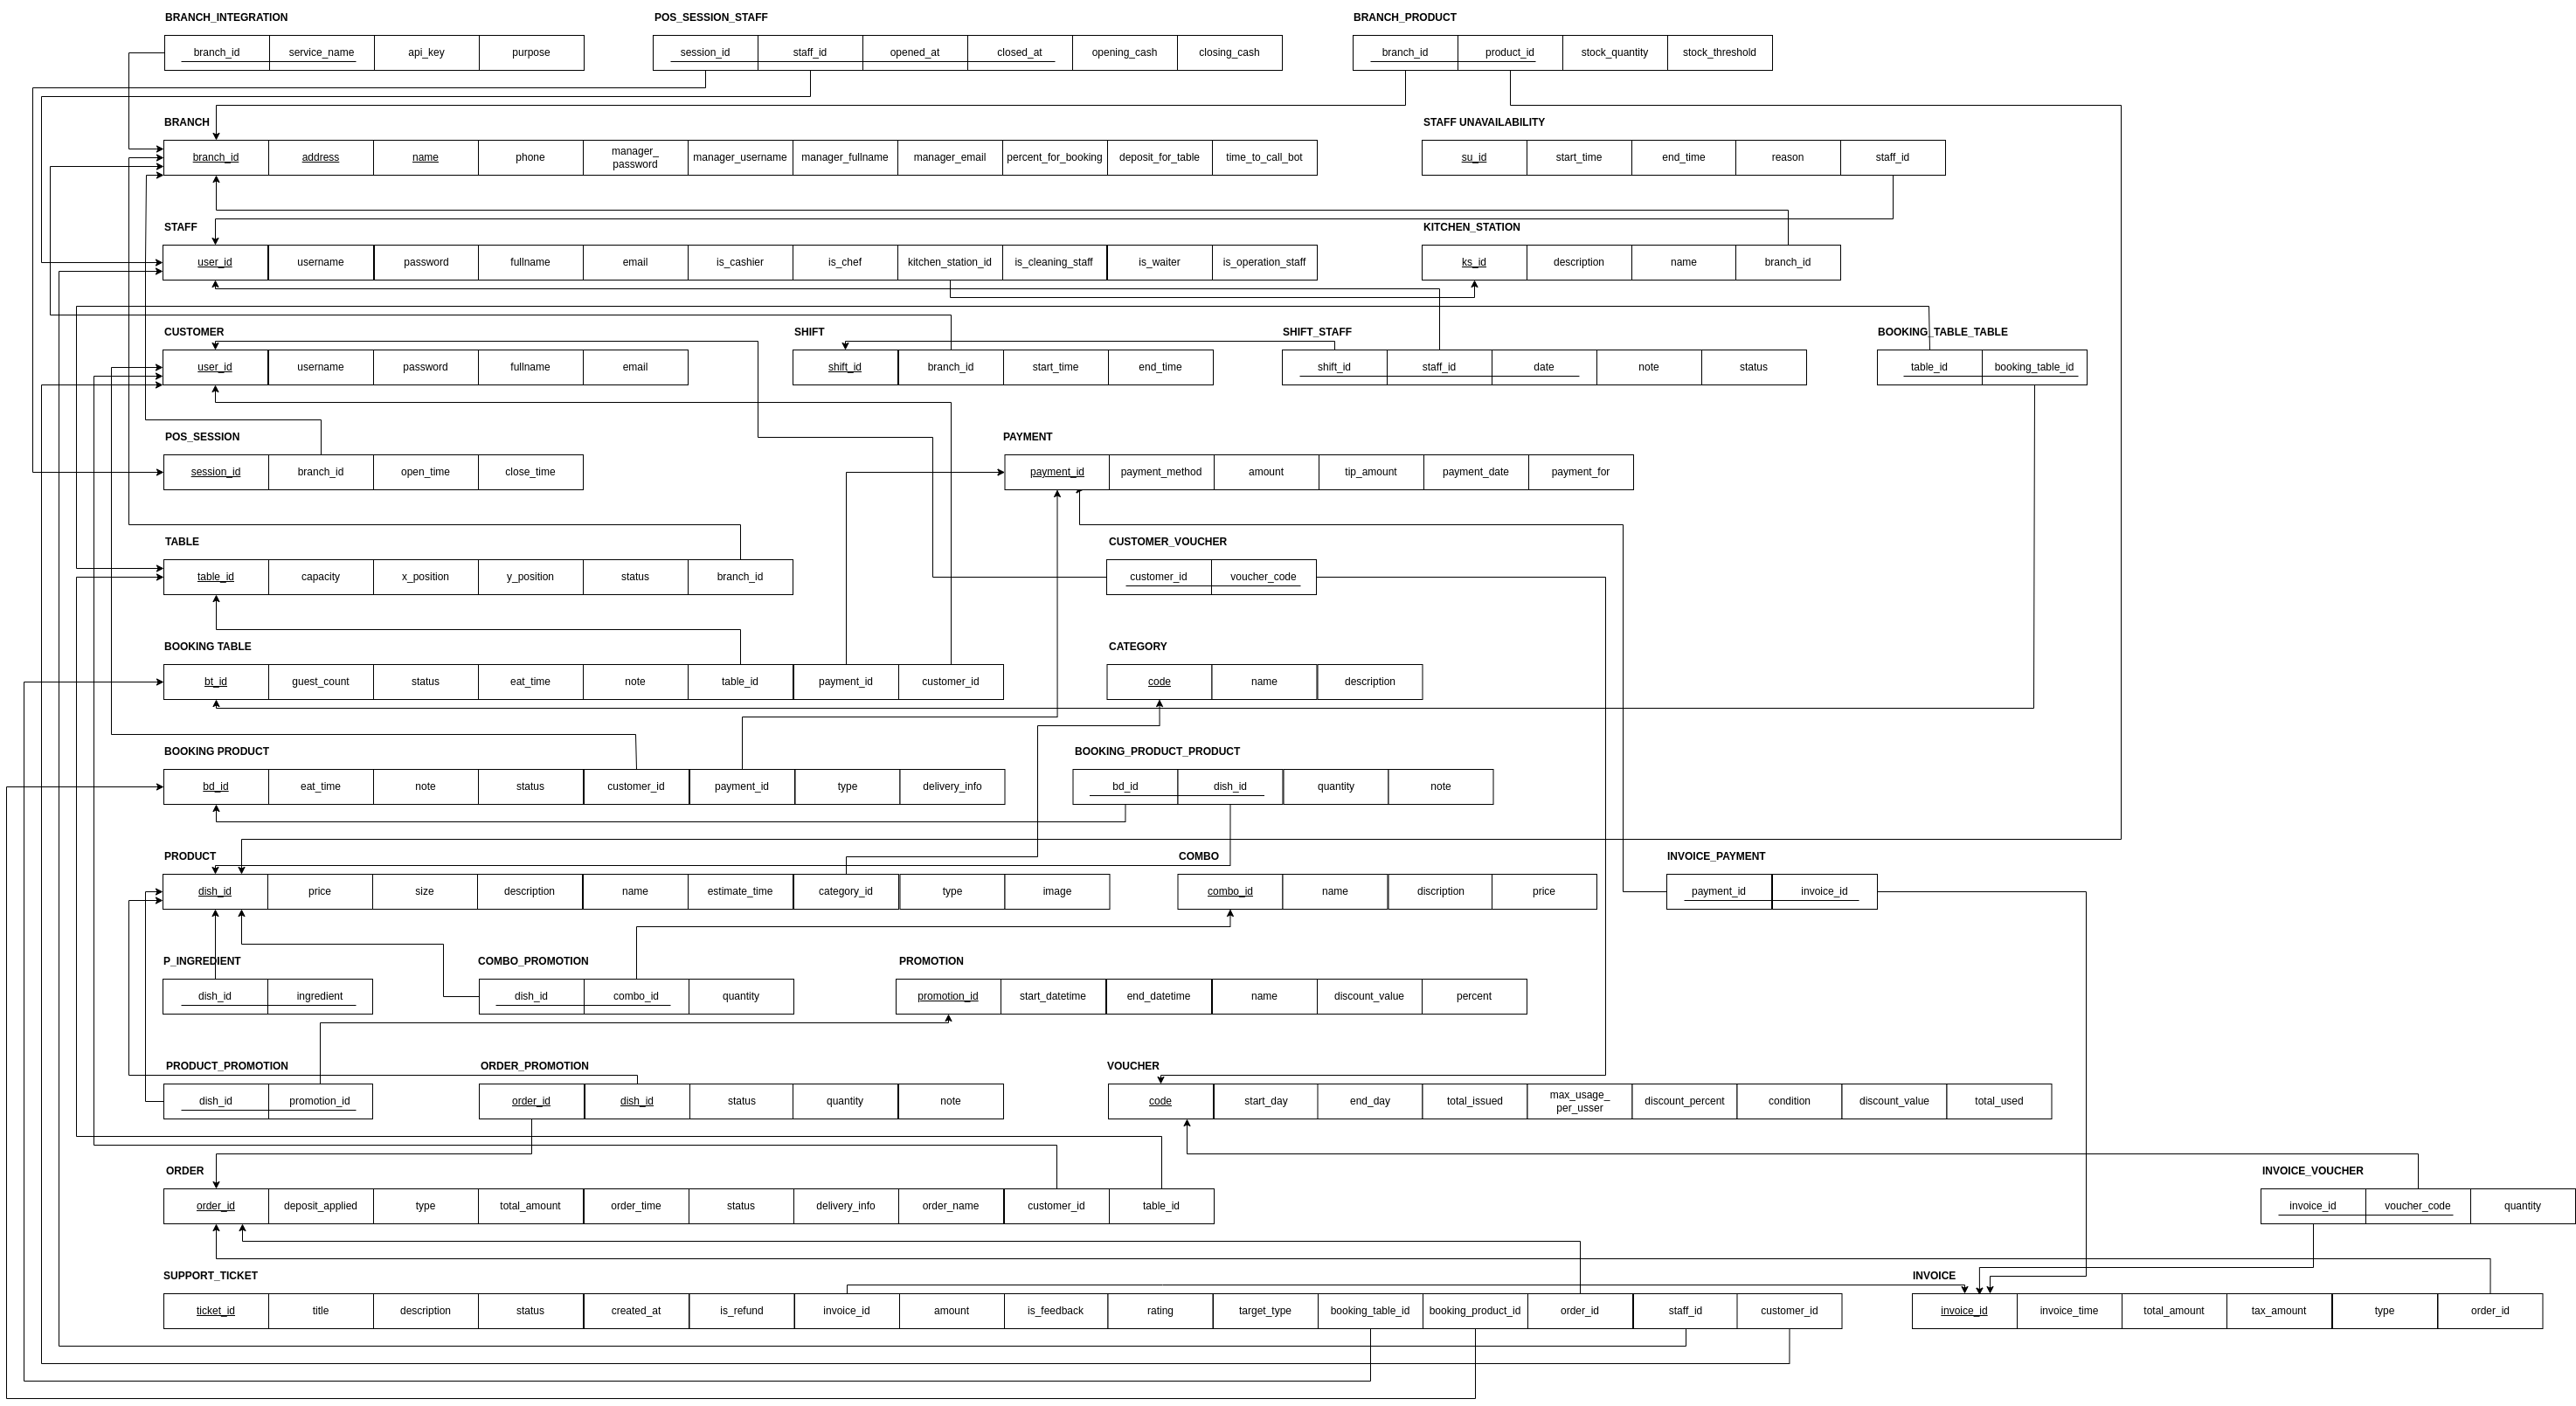
\includegraphics[height=0.9\textheight]{Images/relation.png}
		\vspace{0.5cm}
		\caption{Lược đồ quan hệ cơ sở dữ liệu luận lý}
		\label{fig:my_label}
	\end{figure}

\end{landscape}


\subsubsection{Thiết kế vật lý}

Dưới đây là chi tiết thiết kế vật lý \textbf{một số bảng quan trọng} trong hệ thống. Mỗi bảng thể hiện rõ các thuộc tính, kiểu dữ liệu cụ thể, các ràng buộc và khóa ngoại (nếu có).

\begin{longtable}{|p{3.5cm}|p{3.5cm}|p{7.5cm}|}
	\hline
	\textbf{Thuộc tính} & \textbf{Kiểu dữ liệu} & \textbf{Ràng buộc / CHECK}                                            \\
	\hline
	\endfirsthead

	\hline
	\textbf{Thuộc tính} & \textbf{Kiểu dữ liệu} & \textbf{Ràng buộc / CHECK}                                            \\
	\hline
	\endhead

	% \hline \multicolumn{4}{|r|}{{Còn tiếp ...}} \\
	\hline
	\endfoot

	\hline
	\endlastfoot

	\multicolumn{3}{|l|}{\textbf{product}}                                                                              \\
	\hline
	id                  & bigint                & NOT NULL, PK                                                          \\
	name                & varchar(255)          & NOT NULL                                                              \\
	price               & numeric(38,2)         &                                                                       \\
	type                & varchar(255)          & CHECK IN ('COUNTABLE', 'UNCOUNTABLE', 'SERVICE')                      \\
	category\_id        & bigint                & NOT NULL, FK                                                          \\
	\hline

	\multicolumn{3}{|l|}{\textbf{voucher}}                                                                              \\
	\hline
	id                  & bigint                & NOT NULL, PK                                                          \\
	code                & varchar(100)          & NOT NULL                                                              \\
	discount\_value     & numeric(38,2)         &                                                                       \\
	discount\_percent   & double precision      &                                                                       \\
	start\_date         & date                  & NOT NULL                                                              \\
	end\_date           & date                  & NOT NULL                                                              \\
	\hline

	\multicolumn{3}{|l|}{\textbf{invoice}}                                                                              \\
	\hline
	id                  & bigint                & NOT NULL, PK                                                          \\
	order\_id           & bigint                & NOT NULL, FK                                                          \\
	invoice\_type       & varchar(255)          & CHECK IN ('NORMAL', 'MERGED', 'SPLIT')                                \\
	total\_amount       & numeric(38,2)         &                                                                       \\
	tax\_amount         & numeric(38,2)         &                                                                       \\
	\hline

	\multicolumn{3}{|l|}{\textbf{combo}}                                                                                \\
	\hline
	id                  & bigint                & NOT NULL, PK                                                          \\
	name                & varchar(255)          & NOT NULL                                                              \\
	price               & numeric(38,2)         & NOT NULL                                                              \\
	\hline

	\multicolumn{3}{|l|}{\textbf{orders}}                                                                               \\
	\hline
	id                  & bigint                & NOT NULL, PK                                                          \\
	type                & varchar(255)          & CHECK IN ('DINE\_IN', 'TAKE\_AWAY', 'DELIVERY')                       \\
	oder\_status        & varchar(255)          & CHECK IN ('PLACED', 'PREPARING', 'COMPLETED', 'CANCELLED')            \\
	total\_amount       & numeric(38,2)         &                                                                       \\
	customer\_id        & bigint                & NOT NULL, FK                                                          \\
	\hline

	\multicolumn{3}{|l|}{\textbf{order\_product}}                                                                       \\
	\hline
	id                  & bigint                & NOT NULL, PK                                                          \\
	order\_id           & bigint                & NOT NULL, FK                                                          \\
	product\_id         & bigint                & NOT NULL, FK                                                          \\
	product\_status     & varchar(255)          & CHECK IN ('PENDING', 'PREPARING', 'COMPLETED', 'SERVED', 'CANCELLED') \\
	\hline

	\multicolumn{3}{|l|}{\textbf{restaurant\_table}}                                                                    \\
	\hline
	id                  & bigint                & NOT NULL, PK                                                          \\
	capacity            & integer               &                                                                       \\
	table\_status       & varchar(255)          & CHECK IN ('AVAILABLE', 'OCCUPIED', 'NEEDS\_CLEANING')                 \\
	table\_type         & varchar(255)          & CHECK IN ('STANDARD', 'VIP')                                          \\
	branch\_id          & bigint                & NOT NULL, FK                                                          \\
	\hline

	\multicolumn{3}{|l|}{\textbf{booking\_table}}                                                                       \\
	\hline
	id                  & bigint                & NOT NULL, PK                                                          \\
	booking\_status     & varchar(255)          & CHECK IN ('BOOKED', 'DEPOSIT\_PAID', 'CANCELLED', 'COMPLETED')        \\
	time\_start         & timestamp             & NOT NULL                                                              \\
	time\_end           & timestamp             &                                                                       \\
	customer\_id        & bigint                & NOT NULL, FK                                                          \\
	\hline

	\multicolumn{3}{|l|}{\textbf{booking\_product}}                                                                     \\
	\hline
	id                  & bigint                & NOT NULL, PK                                                          \\
	booking\_status     & varchar(255)          & CHECK IN ('BOOKED', 'DEPOSIT\_PAID', 'CANCELLED', 'COMPLETED')        \\
	booking\_type       & varchar(255)          & CHECK IN ('DINE\_IN','TAKE\_AWAY','DELIVERY')                         \\
	customer\_id        & bigint                & NOT NULL, FK                                                          \\
	branch\_id          & bigint                & NOT NULL, FK                                                          \\
	\hline

	\multicolumn{3}{|l|}{\textbf{combo\_product}}                                                                       \\
	\hline
	id                  & bigint                & NOT NULL, PK                                                          \\
	combo\_id           & bigint                & NOT NULL, FK                                                          \\
	product\_id         & bigint                & NOT NULL, FK                                                          \\
	quantity            & integer               &                                                                       \\
	\hline

	\multicolumn{3}{|l|}{\textbf{invoice\_voucher}}                                                                     \\
	\hline
	id                  & bigint                & NOT NULL, PK                                                          \\
	voucher\_id         & bigint                & NOT NULL, FK                                                          \\
	invoice\_id         & bigint                & NOT NULL, FK                                                          \\
	quantity            & integer               &                                                                       \\
	\hline
\end{longtable}

Sau khi hoàn thiện các bước thiết kế cơ sở dữ liệu từ mô hình khái niệm đến mô hình luận lý và vật lý, hệ thống đã được triển khai trên phần mềm quản lý cơ sở dữ liệu để trực quan hóa quan hệ giữa các bảng. Hình dưới đây thể hiện lược đồ quan hệ đầy đủ của hệ thống cơ sở dữ liệu, được xuất từ công cụ DBeaver sau khi định nghĩa và thiết lập các bảng, khóa chính, khóa ngoại và các liên kết liên quan.

\begin{figure}[H]
	\centering
	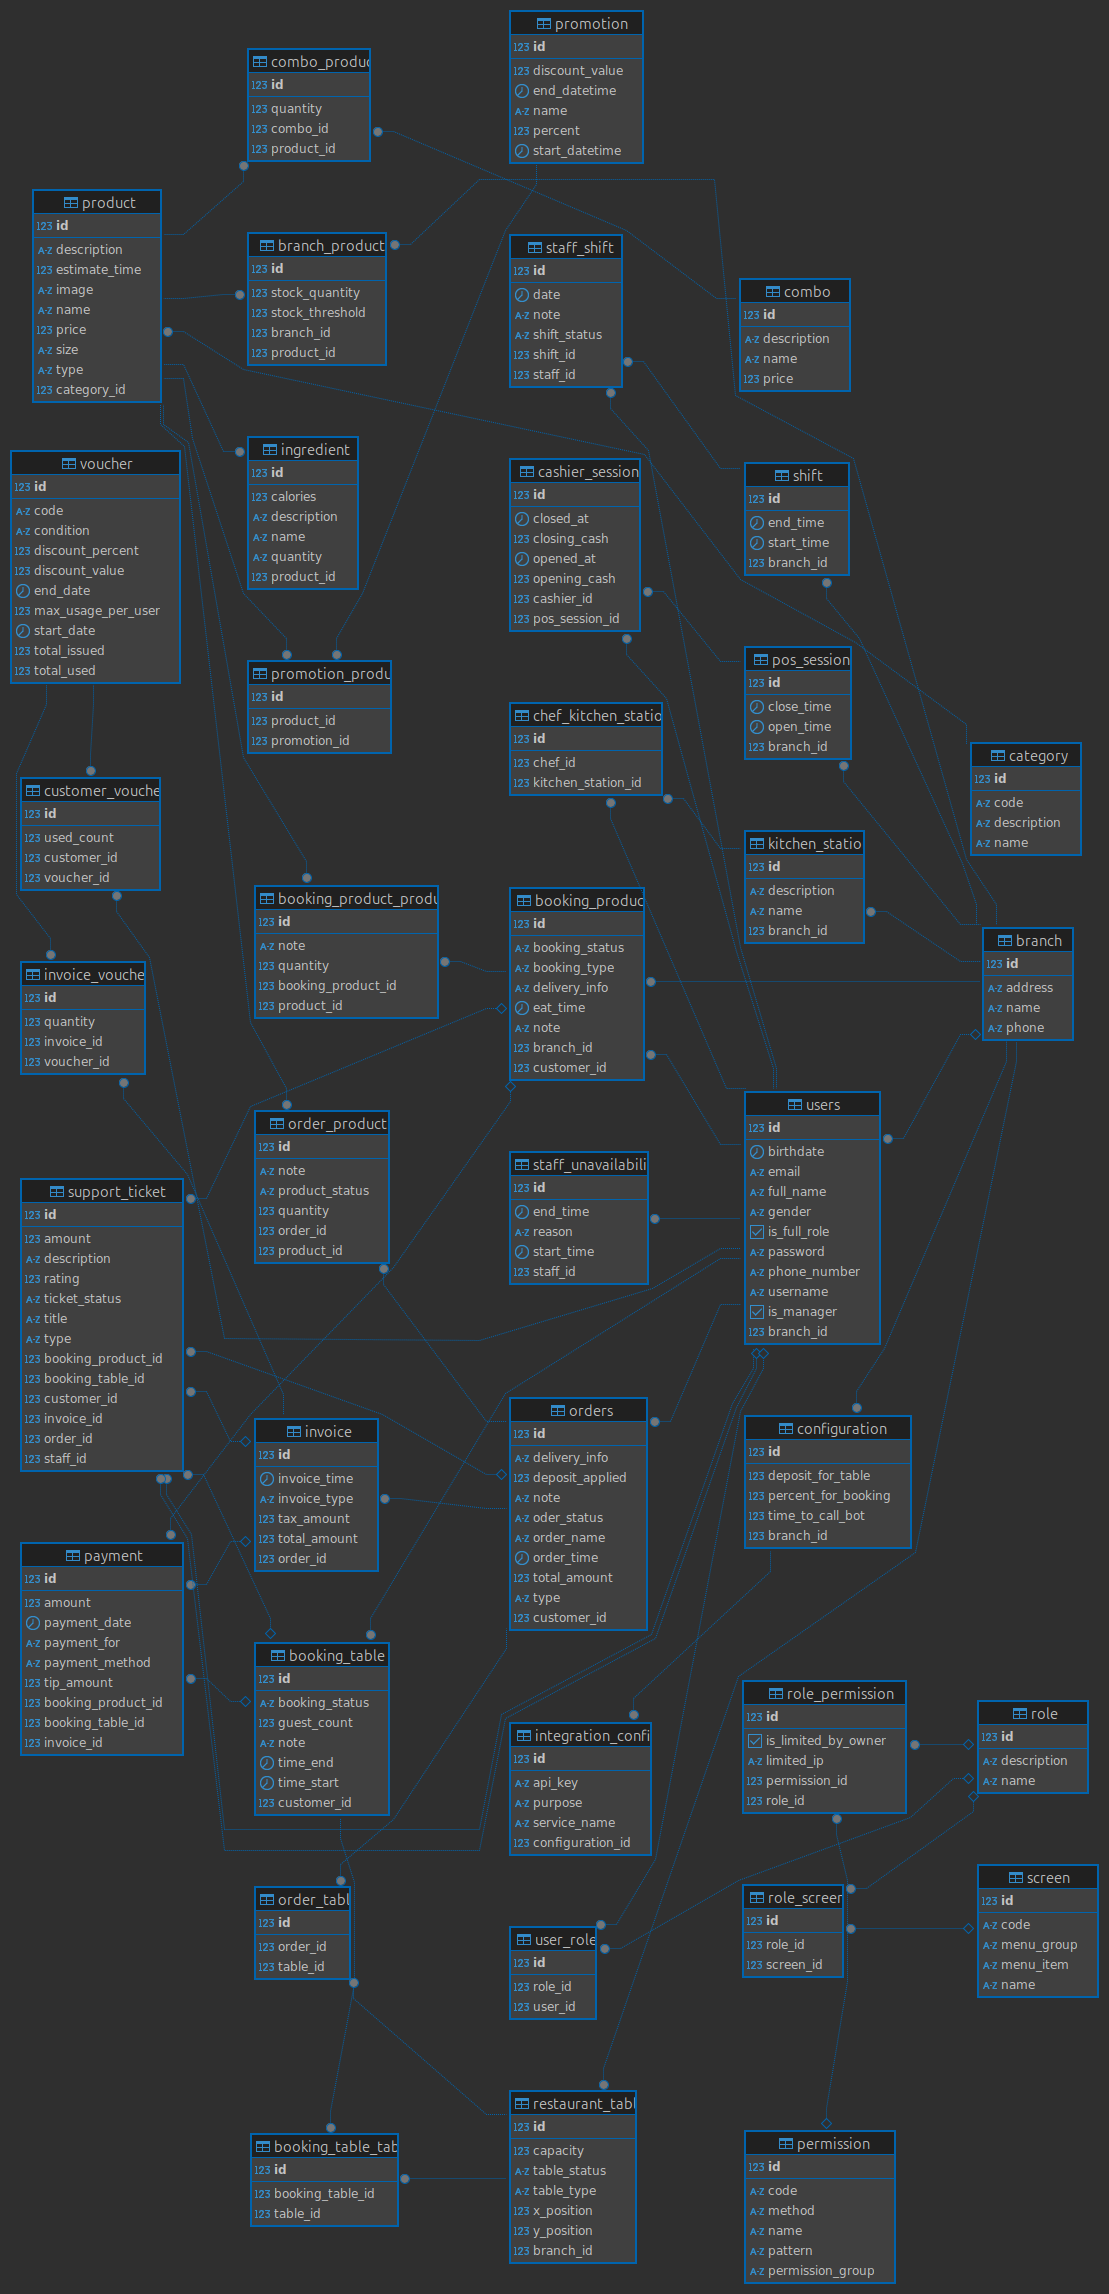
\includegraphics[height=0.9\textheight]{Images/ldqh.png}
	\vspace{0.5cm}
	\caption{Lược đồ quan hệ cơ sở dữ liệu vật lý}
	\label{fig:logical_schema}
\end{figure}